\section{Projection Insertion}
\label{sec:field-reduction}

% Intro/Motivation 
A common optimization in data processing is to early remove intermediate values that are not needed in later phases of the computation. It has been implemented in relational databases for a long time, and has recently been added to the Pig framework. This optimization requires all field accesses in the program to be explicit. A library can provide this, but the usage is more intrusive than if the framework can use compiler support. 

% description of supported types
In \tool we support this optimization for algebraic data types, more specifically final immutable Scala classes with a finite level of nesting. Our approach does not require special syntax or access operators and supports method declarations on a data type like regular Scala classes do. While implementing our benchmarks we found this to be a reasonably expressive model for big data programming. The DSL user needs to supply class declarations, from which we generate all the necessary code for its use in \tool. For these types, LMS describes all field accesses explicitly and we can generate highly specialized code for these types including serialization schemes and other glue code for the back-ends we support.


%\todo{Drop this sentence?}The generated code includes a parsing method, to which the user simply supplies a regular expression, in case the data is stored in text form. 

% explaining the lingo and high level overview of the algorithm.
In section \ref{subsec:lms-optimizations} we have shown how LMS optimizes these classes within the same program scope. However, in \tool we endorse a declarative programming model with many short functions - each having its own scope - as these are easier to read. Each operation in our API has an input type and an output type, and they may have an parameter accepting a closure. 
\todo{explain better}
% Since types support nesting, Field access must be represented as list/seqnce of field accesses to parent types. 
Operations are chained together to form a data flow graph without cycles. \todo{vjovanov does not understand this}We define paths to be the chain of field dereferences needed to access a certain value of an operation's input type. A field access describes such a path, denoted as the chain of dereferences needed on the operation's input. In  figure \ref{fig:type_tree} we show an example. \\
For our projection insertion algorithm we therefore need to analyze all operations to get a list of all field accesses within it. The algorithm goes backwards through the data flow graph and computes for each operation the field reads to propagate them to its predecessors. We use results of this analysis to insert projections before any operation that serializes each object or stores it in memory like the operations \code{cache}, \code{groupByKey} or \code{join}.
 \todo{bit more explanation}
\begin{figure}
% \begin{subfigure}
\begin{lstlisting}[name=code, caption=Types for field access example, captionpos=b, label=lst:types]
case class A(id: String, b: B)
case class B(id: String)  
val t = ("tuple", A("a", B("b"))) 
t: scala.Tuple2[String, A]
\end{lstlisting}
% \end{subfigure}
% \begin{subfigure}
\centering
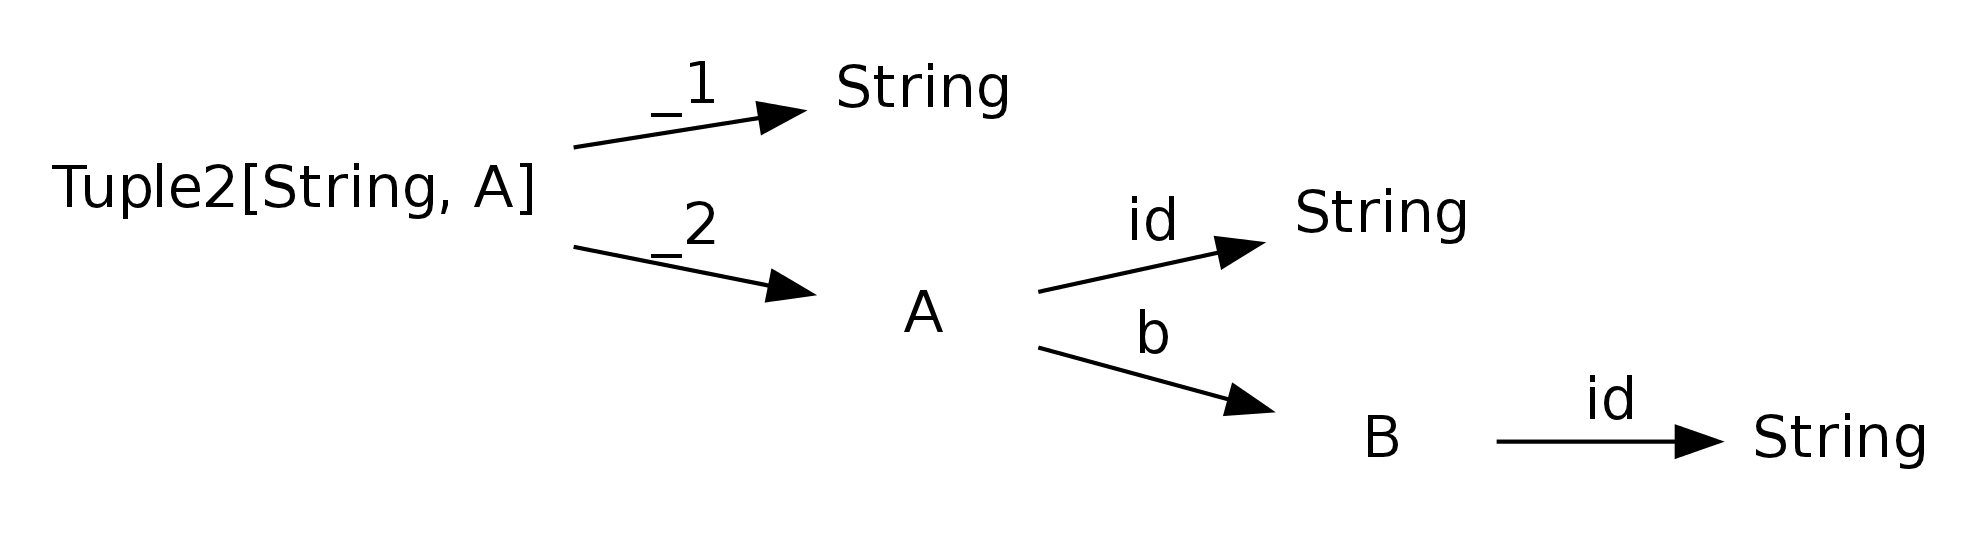
\includegraphics[clip=true, width=0.95\columnwidth]{dot/access.png}
\caption{Visualization of the type. The nodes are the types at each level, the edges describe a field dereference. The leafs are always primitive types, and the path is formed by concatenating the edge labels. An example path description is ``\_2.b.id''}
\label{fig:type_tree}
% \end{subfigure}
\end{figure}
\\
% explaining the analysis

\todo{link it to upstairs}
To analyze one operation we use following primitives:
\begin{itemize}
\item Create field accesses for all fields nested within a type. In \ref{lst:types} a \code{DList.save(....)} on type A generates reads for \code{id} and \code{b.id}. 
\item Rewrite accesses from predecessors according to semantics of the operation. For example, the filter operation will never change the object itself, so all field accesses from a filters successors must be propagated to its predecessors. A GroupByKey operation on the other hand always reads all parts of the key, and additionally changes all field accesses of the form \code{.\_2.iterable.x to .\_2.x}, as the iterable is introduced by the operation itself and is known to conserve the instances.
\item Analyze a closure scope. A closure can be analyzed by filtering all the expressions contained in its scope and checking if they (recursively) read fields from the input of that scope. As such we do not actually analyze all code, analyzing the field reads is enough. 
\item Replace the output symbol of a closure scope with a synthesized one which only contains the later needed fields. See example \todo{sample} for a simple illustration. We need this primitive for the analysis of closures which can do arbitrary transformation, but can reuse it as well for the later projection insertion itself. For a map closure we replace the output, and then analyze the field reads, otherwise some field reads would be in the scope to fill in values into the output which are no longer needed afterwards. This new closure, after dead code elimination, can then be analyzed by the closure analysis primitive.
\end{itemize}
Table \ref{table:field_reduction} shows how these primitives are combined to form the rules of the most important operations on Dlist.\\

Our algorithm depends on DCE and on the \todo{consistent name} structs to array transformation. \todo{SOA} ensures that the last symbol in the scope is always a constructor invocation. When we replace that with a new one, DCE will eliminate the old one. It also uses LMS's optimization that a field read from a constructor invocation bypasses the constructor and reads the value for that field directly.\\
With these preconditions it is sufficient for our algorithm to just analyze the field reads of an input in a certain scope. We do not have to analyze each type of IR node but leave this to the \todo{SOA}language  special case our algorithm understand each language construct, just follow these chains.

% \begin{table}[width=0.5\pagewidth]
    \begin{tabularx}{0.5\textwidth}{l|X|l}
    
        ~            & Field Reads                                                                           & barrier \\ \hline
        filter       & All of successor + closure reads                                                      & ~       \\ 
        flatMap  & All of the closure with a replaced output                                             & ~       \\ 
        map        & All of the closure with a replaced output                                             & ~       \\ 
        join         & Adds accesses to the key, distributes accesses to values to correct predecessor       & x       \\ 
        group by key & Adds access to the key, rewrites accesses to the value's iterable to the value itself & x       \\ 
        reduce       & All accesses from the closure are translated to access of the value's iterable        & ~       \\ 
        save         & Generate accesses for all field reads                                                 & ~       \\ 
        sort         & TODO                                                                                  & TODO    \\ 


    \end{tabularx}
    \label{table:field_reduction}
% \end{table}

